\documentclass{article}
\usepackage[utf8]{inputenc}
\usepackage{amsmath}
\usepackage{amssymb}
\usepackage{geometry}
\usepackage{tikz}

\geometry{margin=0.5in}

\newcommand{\dom}{\operatorname{dom}}

\title{Relational Overriding in Z Notation}
\date{}

\begin{document}

\maketitle

\section{Introduction}

In the \emph{Z} specification language (see, e.g., Spivey~\cite{spivey-z}), \emph{relational overriding}~$\oplus$ updates one partial function with another: wherever the override is defined, its values take precedence; elsewhere, the original mapping is retained. The same idea appears in database theory when merging attribute--value records, with one side winning on overlapping keys.

This note fixes notation, gives a single definition in functional and set-theoretic form, illustrates it with a small table-style example, and lists standard algebraic laws.

\section{Partial functions as rows}

Let $X$ be a set of \emph{attributes} (or keys) and $Y$ a set of \emph{values}. A \emph{row} (or finite map) is modeled as a \emph{partial function}
\[
  f \colon X \nrightarrow Y,
\]
i.e.\ a single-valued relation $f \subseteq X \times Y$. For $x \in \dom f$, we write $f(x)$ for the unique $y$ with $(x,y) \in f$; if $x \notin \dom f$, we say $f$ is \emph{undefined} at~$x$.

In many Z models of tables, ``null'' or ``missing cell'' corresponds to $x \notin \dom f$: the attribute is simply absent from the domain rather than mapped to a distinguished null value.

\section{Domain anti-restriction}

For $S \subseteq X$ and partial $f \colon X \nrightarrow Y$, the \emph{domain anti-restriction} (domain subtraction) $S \vartriangleleft f$ is the partial function obtained by removing from~$f$ every pair whose first component lies in~$S$:
\[
  S \vartriangleleft f
  \;=\;
  \{\, (x,y) \in f \mid x \notin S \,\}.
\]
Equivalently, $\dom(S \vartriangleleft f) = (\dom f) \setminus S$ and values on the remaining domain agree with~$f$.

\section{The overriding operator $\oplus$}

Given partial functions $f,g \colon X \nrightarrow Y$, the \emph{override} $f \oplus g$ is the partial function that behaves like~$g$ on $\dom g$ and like~$f$ on attributes where $g$ is undefined but $f$ is defined.

\subsection{Pointwise definition}

For each $x \in X$,
\begin{equation}
\label{eq:pointwise}
(f \oplus g)(x) =
\begin{cases}
  g(x)      & \text{if } x \in \dom g, \\[0.25em]
  f(x)      & \text{if } x \in \dom f \setminus \dom g, \\[0.25em]
  \text{undefined} & \text{otherwise.}
\end{cases}
\end{equation}
Thus $\dom(f \oplus g) = \dom f \cup \dom g$, and on overlaps $x \in \dom f \cap \dom g$ the value is~$g(x)$: the \emph{right-hand} operand wins.

\subsection{Set-theoretic definition}

Using domain anti-restriction,
\begin{equation}
\label{eq:set}
f \oplus g \;=\; (\dom g \vartriangleleft f) \;\cup\; g.
\end{equation}
First $\dom g \vartriangleleft f$ removes from~$f$ every binding whose key appears in~$g$; then union with~$g$ adds (or replaces with) $g$'s bindings. The same map is obtained as $g \cup (\dom g \vartriangleleft f)$ because the two sets agree on $\dom g$ and are disjoint in the sense needed for single-valued union.

\section{Example: merging two rows}

Let
\begin{itemize}
  \item $T_1 = \{ x \mapsto a,\; y \mapsto b,\; z \mapsto c,\; u \mapsto k \}$,
  \item $T_2 = \{ x \mapsto a,\; y \mapsto d,\; z \mapsto e,\; v \mapsto l \}$.
\end{itemize}
Interpretation: overriding is order-sensitive, so we show both $T_1 \oplus T_2$ and $T_2 \oplus T_1$.

First inspect domains:
\[
  \dom T_1 = \{x,y,z,u\}, \qquad \dom T_2 = \{x,y,z,v\}.
\]
For either order, the result domain is
\[
  \dom(T_1 \oplus T_2) = \dom T_1 \cup \dom T_2 = \{x,y,z,u,v\}.
\]

For $T_1 \oplus T_2$:
\begin{itemize}
  \item $x$ is in both domains, so we take $T_2(x)$;
  \item $y,z$ are also in both domains, so we take $T_2(y),T_2(z)$.
  \item $u$ is only in $T_1$, so it remains $u \mapsto k$.
  \item $v$ is only in $T_2$, so it is added as $v \mapsto l$.
\end{itemize}
Hence
\[
  T_1 \oplus T_2
  = \{ x \mapsto a,\; y \mapsto d,\; z \mapsto e,\; u \mapsto k,\; v \mapsto l \}.
\]
\begin{center}
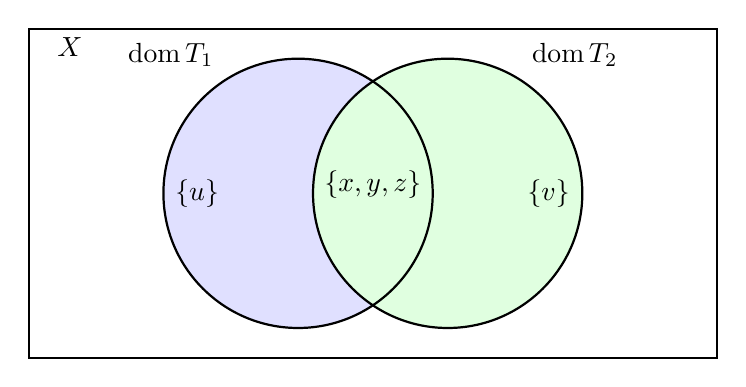
\begin{tikzpicture}[scale=0.95]
  \draw[thick] (-4.6,-2.2) rectangle (4.6,2.2);
  \node[anchor=west] at (-4.35,1.95) {$X$};

  \fill[blue!12] (-1.0,0) circle (1.8);
  \fill[green!12] (1.0,0) circle (1.8);
  \draw[thick] (-1.0,0) circle (1.8);
  \draw[thick] (1.0,0) circle (1.8);

  \node at (-2.7,1.85) {$\dom T_1$};
  \node at (2.7,1.85) {$\dom T_2$};

  \node at (-2.35,0) {$\{u\}$};
  \node at (0,0.12) {$\{x,y,z\}$};
  \node at (2.35,0) {$\{v\}$};
\end{tikzpicture}
\end{center}
\[
  \text{In } T_1 \oplus T_2:\quad
  \{u\}\mapsto \text{from }T_1,\;
  \{x,y,z\}\mapsto \text{from }T_2,\;
  \{v\}\mapsto \text{from }T_2.
\]

For $T_2 \oplus T_1$, the shared keys now take values from $T_1$:
\[
  T_2 \oplus T_1
  = \{ x \mapsto a,\; y \mapsto b,\; z \mapsto c,\; u \mapsto k,\; v \mapsto l \}.
\]
\begin{center}
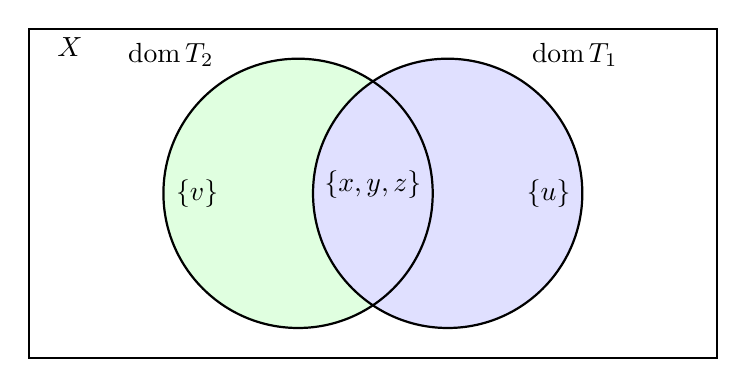
\begin{tikzpicture}[scale=0.95]
  \draw[thick] (-4.6,-2.2) rectangle (4.6,2.2);
  \node[anchor=west] at (-4.35,1.95) {$X$};

  \fill[green!12] (-1.0,0) circle (1.8);
  \fill[blue!12] (1.0,0) circle (1.8);
  \draw[thick] (-1.0,0) circle (1.8);
  \draw[thick] (1.0,0) circle (1.8);

  \node at (-2.7,1.85) {$\dom T_2$};
  \node at (2.7,1.85) {$\dom T_1$};

  \node at (-2.35,0) {$\{v\}$};
  \node at (0,0.12) {$\{x,y,z\}$};
  \node at (2.35,0) {$\{u\}$};
\end{tikzpicture}
\end{center}
\[
  \text{In } T_2 \oplus T_1:\quad
  \{v\}\mapsto \text{from }T_2,\;
  \{x,y,z\}\mapsto \text{from }T_1,\;
  \{u\}\mapsto \text{from }T_1.
\]
So on shared keys, the right-hand map wins; on non-shared keys, whichever side defines the key contributes it.

Equation~\eqref{eq:set} gives both orders:
\[
  T_1 \oplus T_2 = (\dom T_2 \vartriangleleft T_1) \cup T_2.
\]
Because $\dom T_2=\{x,y,z\}$, anti-restriction removes from $T_1$ exactly the pairs with keys $x,y,z$:
\[
  \dom T_2 \vartriangleleft T_1 = \{u \mapsto k\},
\]
so
\[
  T_1 \oplus T_2 = \{u \mapsto k\} \cup T_2
  = \{ x \mapsto a,\; y \mapsto d,\; z \mapsto e,\; u \mapsto k,\; v \mapsto l \}.
\]
Similarly,
\[
  T_2 \oplus T_1 = (\dom T_1 \vartriangleleft T_2) \cup T_1
  = \{v \mapsto l\} \cup T_1
  = \{ x \mapsto a,\; y \mapsto b,\; z \mapsto c,\; u \mapsto k,\; v \mapsto l \}.
\]

\section{Algebraic properties}

For all suitable partial $f,g,h$ (and empty map $\emptyset$):
\begin{enumerate}
  \item \textbf{Non-commutativity.} In general $f \oplus g \neq g \oplus f$; the right operand takes precedence on $\dom f \cap \dom g$.
  \item \textbf{Associativity.} $(f \oplus g) \oplus h = f \oplus (g \oplus h)$.
  \item \textbf{Right identity and left identity for $\emptyset$.}
        $f \oplus \emptyset = f$ and $\emptyset \oplus f = f$.
  \item \textbf{Idempotence.} $f \oplus f = f$.
\end{enumerate}

\begin{thebibliography}{9}
\bibitem{spivey-z}
J.~M. Spivey,
\emph{The Z Notation: A Reference Manual},
Prentice Hall International (UK) Ltd., 2nd edition, 1992.
\end{thebibliography}

\end{document}
